\documentclass[runningheads,a4paper]{llncs}

\usepackage[american]{babel}
\usepackage[utf8]{inputenc}


%better font, similar to the default springer font
%cfr-lm is preferred over lmodern. Reasoning at http://tex.stackexchange.com/a/247543/9075
\usepackage[%
rm={oldstyle=false,proportional=true},%
sf={oldstyle=false,proportional=true},%
tt={oldstyle=false,proportional=true,variable=true},%
qt=false%
]{cfr-lm}
%
%if more space is needed, exchange cfr-lm by mathptmx
%\usepackage{mathptmx}

\usepackage{graphicx}

%extended enumerate, such as \begin{compactenum}
\usepackage{paralist}

\usepackage{float}

%put figures inside a text
%\usepackage{picins}
%use
%\piccaptioninside
%\piccaption{...}
%\parpic[r]{\includegraphics ...}
%Text...

%Sorts the citations in the brackets
\usepackage{cite}

\usepackage[T1]{fontenc}

%for easy quotations: \enquote{text}
\usepackage{csquotes}

%enable margin kerning
\usepackage{microtype}

%tweak \url{...}
\usepackage{url}
%nicer // - solution by http://tex.stackexchange.com/a/98470/9075
\makeatletter
\def\Url@twoslashes{\mathchar`\/\@ifnextchar/{\kern-.2em}{}}
\g@addto@macro\UrlSpecials{\do\/{\Url@twoslashes}}
\makeatother
\urlstyle{same}
%improve wrapping of URLs - hint by http://tex.stackexchange.com/a/10419/9075
\makeatletter
\g@addto@macro{\UrlBreaks}{\UrlOrds}
\makeatother

%diagonal lines in a table - http://tex.stackexchange.com/questions/17745/diagonal-lines-in-table-cell
%slashbox is not available in texlive (due to licensing) and also gives bad results. This, we use diagbox
%\usepackage{diagbox}

%required for pdfcomment later
\usepackage{xcolor}

% new packages BEFORE hyperref
% See also http://tex.stackexchange.com/questions/1863/which-packages-should-be-loaded-after-hyperref-instead-of-before

%enable hyperref without colors and without bookmarks
\usepackage[
%pdfauthor={},
%pdfsubject={},
%pdftitle={},
%pdfkeywords={},
bookmarks=false,
breaklinks=true,
colorlinks=true,
linkcolor=black,
citecolor=black,
urlcolor=black,
%pdfstartpage=19,
pdfpagelayout=SinglePage,
pdfstartview=Fit
]{hyperref}
%enables correct jumping to figures when referencing
\usepackage[all]{hypcap}

%enable nice comments
\usepackage{pdfcomment}
\newcommand{\commentontext}[2]{\colorbox{yellow!60}{#1}\pdfcomment[color={0.234 0.867 0.211},hoffset=-6pt,voffset=10pt,opacity=0.5]{#2}}
\newcommand{\commentatside}[1]{\pdfcomment[color={0.045 0.278 0.643},icon=Note]{#1}}

%compatibality with TODO package
\newcommand{\todo}[1]{\commentatside{#1}}

%enable \cref{...} and \Cref{...} instead of \ref: Type of reference included in the link
\usepackage[capitalise,nameinlink]{cleveref}
%Nice formats for \cref
\crefname{section}{Sect.}{Sect.}
\Crefname{section}{Section}{Sections}
\crefname{figure}{Fig.}{Fig.}
\Crefname{figure}{Figure}{Figures}

\usepackage{xspace}
%\newcommand{\eg}{e.\,g.\xspace}
%\newcommand{\ie}{i.\,e.\xspace}
\newcommand{\eg}{e.\,g.,\ }
\newcommand{\ie}{i.\,e.,\ }

%introduce \powerset - hint by http://matheplanet.com/matheplanet/nuke/html/viewtopic.php?topic=136492&post_id=997377
\DeclareFontFamily{U}{MnSymbolC}{}
\DeclareSymbolFont{MnSyC}{U}{MnSymbolC}{m}{n}
\DeclareFontShape{U}{MnSymbolC}{m}{n}{
    <-6>  MnSymbolC5
   <6-7>  MnSymbolC6
   <7-8>  MnSymbolC7
   <8-9>  MnSymbolC8
   <9-10> MnSymbolC9
  <10-12> MnSymbolC10
  <12->   MnSymbolC12%
}{}
\DeclareMathSymbol{\powerset}{\mathord}{MnSyC}{180}

% correct bad hyphenation here
\hyphenation{op-tical net-works semi-conduc-tor}




\newcommand*{\captionsource}[2]{%
  \caption[{#1}]{%
    #1%
    \\\hspace{\linewidth}%
    \textbf{Source:} #2%
  }%
}


\begin{document}

%Works on MiKTeX only
%hint by http://goemonx.blogspot.de/2012/01/pdflatex-ligaturen-und-copynpaste.html
%also http://tex.stackexchange.com/questions/4397/make-ligatures-in-linux-libertine-copyable-and-searchable
%This allows a copy'n'paste of the text from the paper
\input glyphtounicode.tex
\pdfgentounicode=1


%%%%%%%%%%%%%%%%%%%%%




\title{Overview of Semi-Supervised Learning}
%If Title is too long, use \titlerunning
%\titlerunning{Short Title}

%Single insitute
\author{Felix Jankowski}
%If there are too many authors, use \authorrunning
%\authorrunning{First Author et al.}
\institute{Universität Augsburg - Seminar: Machine Learning und User Interfaces}

%Multiple insitutes
%Currently disabled
%
\iffalse
%Multiple institutes are typeset as follows:
\author{Firstname Lastname\inst{1} \and Firstname Lastname\inst{2} }
%If there are too many authors, use \authorrunning
%\authorrunning{First Author et al.}

\institute{
Insitute 1\\
\email{...}\and
Insitute 2\\
\email{...}
}
\fi

\maketitle

\begin{abstract}
Die heutige Gesellschaft wäre ohne Machine Learning nicht denkbar. Nicht nur wäre der Zugang zu Informationen begrenzt, auch Branchen wie die Pharmazie verdanken dieser Technologie ihre wesentlichen Fortschritte der letzten Jahre.
Dabei kann zwischen Supervised und Unsupervised Learning differenziert werden, je nachdem, ob korrekte Outputwerte zum Training vorhanden sind oder nicht.
Oft wäre es jedoch hilfreich und effektiv, wenn selbstlernende Algorithmen  beide Methoden kombinieren könnten. Dies ist das Ziel von Semi-Supervised Learning. Um die dahinterstehenden Prizipien zu verstehen, wird in diesem Paper zunächst das Prinzip von Supervised und Unsupervised Learning erklärt. Darauf aufbauend wird die Funktionsweise von Semi-Supervised Learning erläutert.\end{abstract}

%\keywords{...}



%%%%%%%%%%%%%%%%%%%%%%%%%%%%%%%%%%%%%%%%%%%%%%%%%%%%%%%%%%%%%%%%%%%%%%%%%%%%%%%
\section{Einführung in das Machine Learning}\label{sec:intro}
%%%%%%%%%%%%%%%%%%%%%%%%%%%%%%%%%%%%%%%%%%%%%%%%%%%%%%%%%%%%%%%%%%%%%%%%%%%%%%%

So gut wie jeder benutzt täglich Produkte, die Ergebnisse mittels Machine Learning generieren. Die meisten von uns, ohne es zu wissen. Ob Produktvorschläge im Newsletter von Amazon, personalisierte Werbung auf Facebook oder eine schlichte Google-Suche; an all diesen Stellen haben selbstlernende Algorithmen längst von Menschen erdachte Berechnungsverfahren abgelöst\cite{Coursera}. Kennzeichen hierbei ist, dass ein Computer Entscheidungen nicht mittels von Menschen vorab entwickelter Verfahren trifft, sondern aus einer großen Anzahl von Beispielen selbstständig lernt und hieraus erworbenes Wissen verallgemeinert.\cite{wiki:Machine_learning}


\begin{figure} [ht]
  \centering
  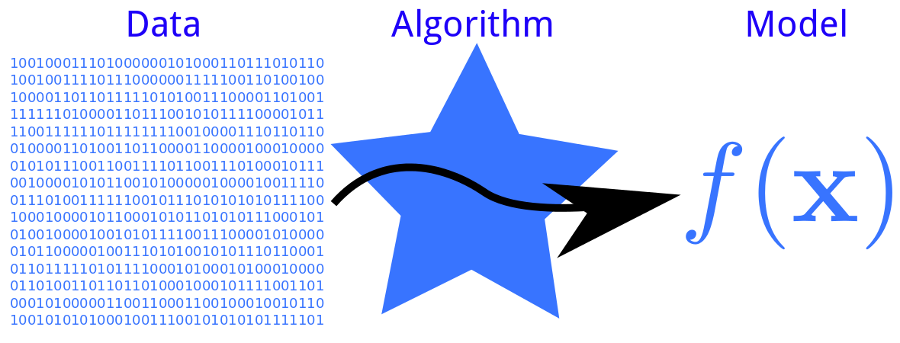
\includegraphics[width=0.8\textwidth]{res/ml-900.png}
    	%\caption{Machine Learning: Ein Modell wird durch einen Algorithmus generiert }
      \captionsource{Machine Learning: Ein Modell wird durch einen Algorithmus generiert}{\cite{Phili47:online}}

    %\source{\ref{},\cite{} or free Text}
  \label{fig:overview}
\end{figure}

Mittlerweile gibt es Startups wie "BigML, Inc", die Machine Learning für jedermann \emph{as a service} anbieten, ohne dass Kenntnisse der Verfahren und Algorithmen nötig wären: \cite{BigML33:online}

Dieses Produkt hat der Autor als Programmierer der IT-Abteilung des Berliner Finanzdienstleisters "Decimo GmbH" im Januar 2016 erfolgreich als Alternative zu den vorhandenen und von Finanzmathematikern zur Betrugserkennung entwickelten Risikomodellen getestet. Anstelle mühsam Zusammenhänge zu erkunden, darin Risikofaktoren zu Extrahieren und zu Gewichten und manuell eine Entscheidungsschwelle festzulegen, wurden hier pseudonymisierte Daten zu 3000 Transaktionen, darunter 75 Betrugsfälle an eine API übermittelt, aus denen serverseitig ein Entscheidungsgraph generiert wird. Weitere 1000 Transaktionen mit 15 Betrugsfällen wurden zum statistischen Testen verwendet.

\subsection{Supervised Learning}

Sämtliche von Decimo übermittelten Transaktionen waren bereits abgeschlossen, weshalb bei allen bereits bekannt war, ob es sich um einen Betrugsfall gehandelt hatte. In diesem Fall spricht man von \emph{labeled data}.

Bei der Zuordnung von Daten in diskrete, vorab festgelegte Klassen handelt es sich um eine Form des \emph{supervised learning}s, formal definiert durch:

\enquote{In supervised learning, the training set consists of a set of $n$ ordered pairs $(x_1, y_1),(x_2, y_2), ...,(x_n, y_n)$, where each $x_i$ is some measurement or set of measurements of a single example data point, and $y_i$ is the label for that data point. (...) The test data in supervised learning is another set of m measurements without
labels: $(x_{n+1}, x_{n+2}, ..., x_{n+m})$.} \cite{miller}

Im oben verwendeten Beispiel der Betrugserkennung wäre $y$ für alle betrügerischen Transaktionen $1$, in allen Fällen $0$.

Weitere Beispiele für \emph{supervised learning} sind die Schätzung des Geschlechts von Menschen oder Tieren anhand von Körpergröße und Gewicht (Klassifikation in männlich oder weiblich) \cite{zhu_goldberg_2009}, die Berechnung eines Marktpreises für Häuser aus Parametern wie z.B. Baujahr und Wohnfläche mittels Regression \cite{Coursera} oder die Erkennung von Handschriften durch Neuronale Netzwerke, bei der jeder Buchstabe einer Position im Alphabet zugeordnet wird.

%Die größte Schwäche von BigML, Konfidenzintervalle



\subsection{Unsupervised Learning}

Häufig existieren jedoch Probleme, für die im Voraus keine Ergebnisse bekannt sind. Ziel beim \emph{unsupervised learning} ist es, Muster in den Daten zu erkennen, die von einer rein zufälligen Verteilung abweichen\cite{Ghahramani04unsupervisedlearning}.

\enquote{ Unsupervised learning algorithms work on a training sample with $n$ instances $\{x_i\}_{i=1}^n$. There is no teacher providing supervision as to how individual instances should be handled — this is the defining property of unsupervised learning.}\cite{zhu_goldberg_2009}


\begin{figure} [ht]
  \centering
  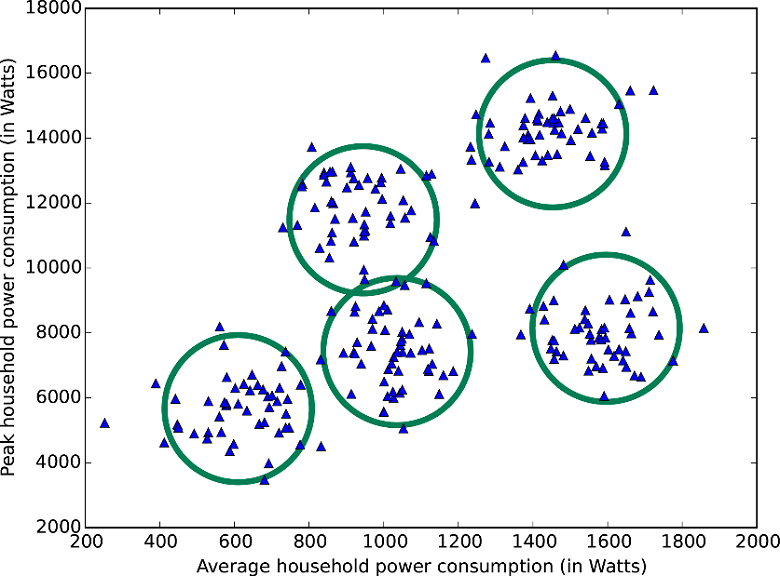
\includegraphics[width=0.9\textwidth]{res/classification.png}
      \captionsource{Clustering: Typische Anwendung von unsupervised learning}{\cite{Howto22:online}}
  \label{fig:cluserting}
\end{figure}


Wichtigste Anwendung des \emph{unsupervised learning}s ist das \emph{Clustering}, bei dem versucht wird, die Daten in sinnvolle, nicht vorher definierte Gruppen, einzuteilen. Je nach Algorithmus und Anwendungsfall wir die Anzahl der Gruppen vorher extern festgelegt oder vom Algorithmus nach mathematischen Prinzipien bestimmt. 

Ebenfalls häufig verwendet wird die \emph{dimensionality reduction}, bei der korrelierende Eigenschaften zur Verringerung von Datenmenge und Rechenzeiten entfernt werden.

\section{Semi-Supervised Learning}

Inzwischen wurden Verfahren entwickelt, die zum Training sowohl Daten, bei denen der korrekte Funktionswert bekannt ist als auch ungelabelte Daten verwenden. Diese lassen sich folglich keiner der beiden Kategorien zuordnen, weswegen die Zwischenkategorie \emph{Semi-Supervised Learning} geschaffen wurde. 

Beispielsweise lässt sich bei der Entwicklung von SPAM-Filtern beobachten, dass Nutzer diese E-Mails tatsächlich nur sehr selten als \enquote{unerwünscht} markieren. Aufgrund der Vielzahl der Variationen (Phishing, Werbung, Betrug, Trojaner, etc.) und der Menge der verschiedenen Wörtern in einer Sprache ist jedoch gerade hier ein umfangreiches Trainingsset notwendig.

Daneben besteht eine große Anzahl ähnlicher Probleme. In vielen Fällen existiert eine gigantische Menge an Daten, jedoch gestaltet dich die Gewinnung passender Labels aufwändig oder schwierig, da dies manuelle Arbeit voraussetzt.

Deutlich wird dies bei der automatische Erkennung von natürlicher Sprache. Beispielsweise findet sich im Videoportal \emph{YouTube} nahezu unbegrenzt frei verfügbare Stimmaufzeichnungen verschiedenster Sprecher, jedoch existieren  Transkriptionen oder Untertitel, anhand derer die Algorithmen zur Spracherkennung trainiert werde könnten, nur äußerst spärlich. 

Die Lösung vergleichbarer Probleme ist das Ziel von \emph{Semi-Supervised Learning}.


\subsection{Wie funktioniert Semi-Supervised Learning}

Die meisten Algorithmen dieser Art stellen eine dahingehende Erweiterung bestehender Verfahren des \emph{supervised} oder \emph{unsupervised learnings} dar, dass zusätzliche Information der jeweils anderen Kategorie mitberücksichtigt werden kann.

Interessanterweise ähnelt dies dem Spracherwerb von Kleinkindern. Nach den ersten Wörtern \enquote{Mama} und \enquote{Papa} werden in der Regel zunächst Nomen, meist Kategoriebezeichnungen wie z.B. \enquote{Hund}, \enquote{Katze}, \enquote{Haus} erlernt. Ist ein Kind auf ein Objekt fokussiert, wird instinktiv von den Begleitpersonen der passende Begriff genannt. Irgendwann entdeckt das Kind Ähnlichkeiten und Zusammenhänge und ruft begeistert das passende Wort, sobald es ein Objekt zugeordnet hat. Mit der Zeit wird dadurch die externe Kategorisierung durch Mustererkennung ersetzt.\cite{zhu_goldberg_2009}

In \ref{fig:ss-clust} ist ein \cite{zhu_goldberg_2009} entnommenes Beispiel für \emph{semi-supervised clustering} abgebildet, bei dem Daten durch den ein-dimensionalen Messwert $x$ der Klasse \emph{positiv} (+) oder \emph{negativ} (-) zugeordnet werden. 

\begin{figure} [ht]
  \centering
  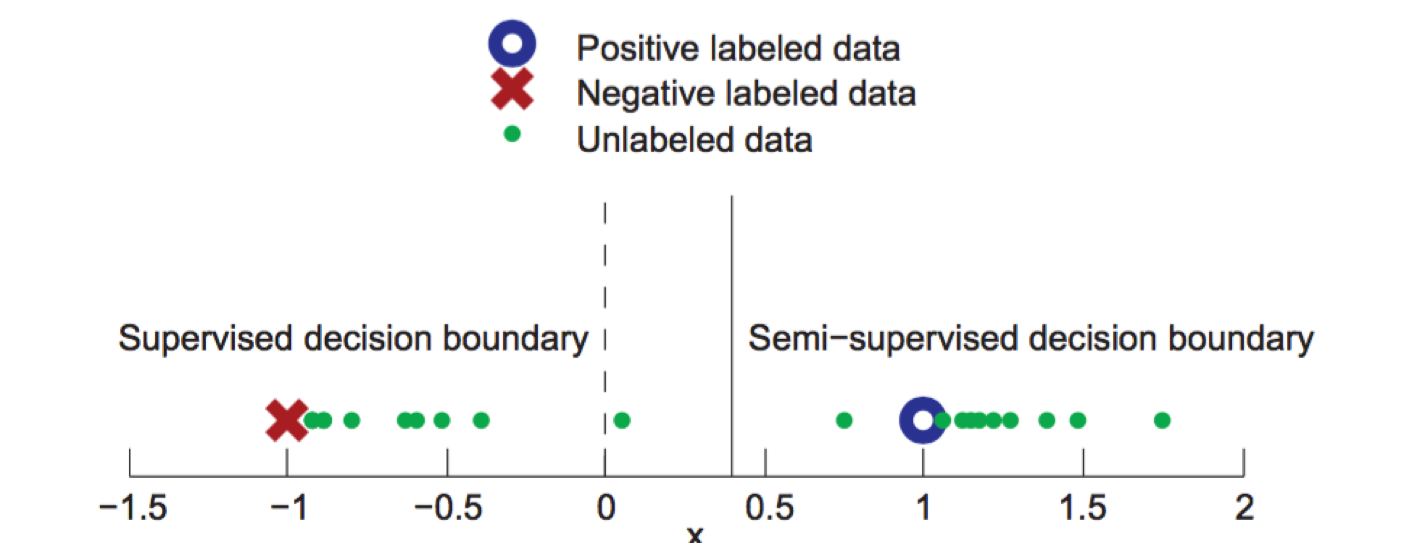
\includegraphics[width=1\textwidth]{res/ss_classification.png}
      \captionsource{Beispiel für semi-supervised classification}{\cite{zhu_goldberg_2009}}
  \label{fig:ss-clust}
\end{figure}


Bei einem aus nur zwei gelabelten Punkten bestehenden Trainingsset ($x_1 = -1; y_1 = -$ und $x_2 = 1; y_2 = +$), würde ein supervised learning Algorithmus die Entscheidungsschwelle beim arithmetische Mittel, in diesem Falle $x_b = 0$ festlegen. Sämtliche Messwerte mit $x > 0$ würden der Klasse \emph{positiv} zugeordnet.

Im Gegensatz zu einem Computer würde ein Mensch in der Abbildung sofort ein Muster erkennen und vermuten, dass es sich beim x-Wert von Punkt 1 nicht um dem Durchschnitt der Klasse \emph{negativ}, sondern im Gegenteil um einen Minimum handelt.

Beim \emph{Semi-Supervised Learning} werden die anderen Punkte, für die kein y-Wert bekannt ist, mit berücksichtigt. Zunächst könnten diese Punkte, z.B. über den \emph{k-Means Algorithmus} ebenfalls in die Klassen + oder - eingeordnet werden. Durch das hierdurch entstehende, deutlich umfangreichere Trainingsset, lässt sich eine Schwelle bei $x_b \approx 0.4$ errechnen, welche auch der menschlichen Intuition entspricht.


\subsection{Verschiedene Arten des Semi-Supervised Learning}


Prinzipiell lassen sich zwei verschiedene Verfahren unterscheiden\cite{zhu_goldberg_2009}: 

\begin{enumerate}

\item \textbf{Semi-supervised classification:} Hierbei werden wie oben beschrieben die bekannten Methoden zur Klassifikation verbessert. Das Trainingsset $\{(x_i, y_i)\}_{i=1}^l, \{x_j\}_{j=l+1}^{l+u}$  besteht aus einer Anzahl $l$ von gelabelten und einer Anzahl $n$ an nicht-gelabelten Daten. Nicht zwingend, aber in der Regel liegen wesentlich mehr ungelabelte Daten vor, d.h. $u \gg l$. Hierbei ist das Ziel durch Nutzbarmachung der ungelabelten Daten mit einem größeren Trainingsset die Genauigkeit der Vorhersagefunktion $f$ auf künftigen Daten zu erhöhen.

\item  \textbf{Constrained clustering:} Im Gegensatz zum normalen Clustering, bei dem lediglich die ungelabelten Daten $\{x_i\}_{i=1}^n$ vorliegen, kann hier weitere Information verarbeitet werden. Beispielsweise kann dem Algorithmus mitgeteilt werden, dass bestimmte Werte $x_i, x_j$ dem selben oder unterschiedlichen Clustern angehören (sog. \emph{must-link}) oder die Anzahl der maximalen Elemente pro Cluster kann begrenzt werden.
  

\end{enumerate}


\subsection{Induktive und Transduktive Algorithmen}

In Kapitel 1 wurden zwei verschiedene Arten von Algorithmen behandelt. Beim \emph{supervised learning} waren für alle Werte bereits Ergebnisse vorhanden, so dass eine möglichst zuverlässige Berechnungsmethode für künftige Werte gesucht wird. 
Hingegen wurde beim \emph{unsupervised learning}, wie beispielsweise beim Gruppieren in verschiedene Klassen ausschließlich auf bestehenden Daten der Vergangenheit gearbeitet.

Interessanterweise können mit \emph{semi-supervised learning} beide Ziele verfolgt werden, auch wenn hier ein Teil des Trainingssets aus ungelabelten Daten besteht. Möchte man lediglich diesem Teil ebenfalls Labels zuweisen, spricht man von \emph{Transduktivem Lernen}. Formal wird durch das Trainingsset $\{(x_i, y_i)\}_{i=1}^l, \{x_j\}_{j=l+1}^{l+u}$ eine Funktion berechnet, die den bisher ungelabelten Daten die Labels $\{y_j\}_{j=l+1}^{l+u}$ zuweist.

Im oben genannten Beispiel \ref{fig:ss-clust} war jedoch das Ziel, ein Entscheidungsverfahren für künftige Werte zu finden. In diesem Fall spricht man von induktiven Verfahren. Dies ist dadurch definiert, dass mit Hilfe des Trainingssets $\{(x_i, y_i)\}_{i=1}^l, \{x_j\}_{j=l+1}^{l+u}$ eine allgemeine Funktion $f : X \mapsto Y$ berechnet wird, die auch für $\forall X \notin \{x_j\}_{j=l+1}^{l+u}$ gute Ergebnisse liefert.

Wie auch beim \emph{supervised learning} kann die Qualität dieser Funktion durch ein Testset $\{(x_k, y_k)\}_{k=1}^m$, welches nicht Teil des Trainingssets ist bewertet werden. Zum Vergleich der Qualität ist der sog. $F_1-Wert$ gebräuchlich.\cite{zhu_goldberg_2009}



\subsection{Probleme und Schwächen}

Leider ist es unvermeidlich, dass durch Übernahme der Methoden aus beiden Kategorien auch ein Teil der Schwächen mitübernommen wird. 

Beispielsweise zeigen die \cite{zhu_goldberg_2009} entnommenen Abbildungen \ref{fig:cav1} und \ref{fig:cav2} wie bei der Klassifikation durch \emph{1-nearest-neighbour} bereits ein einzelner Ausreißer die gesamten Ergebnisse zerstören kann, sofern die Daten nicht in deutlich voneinander abgegrenzten Clustern liegen.


\begin{figure} [H]
  \centering
  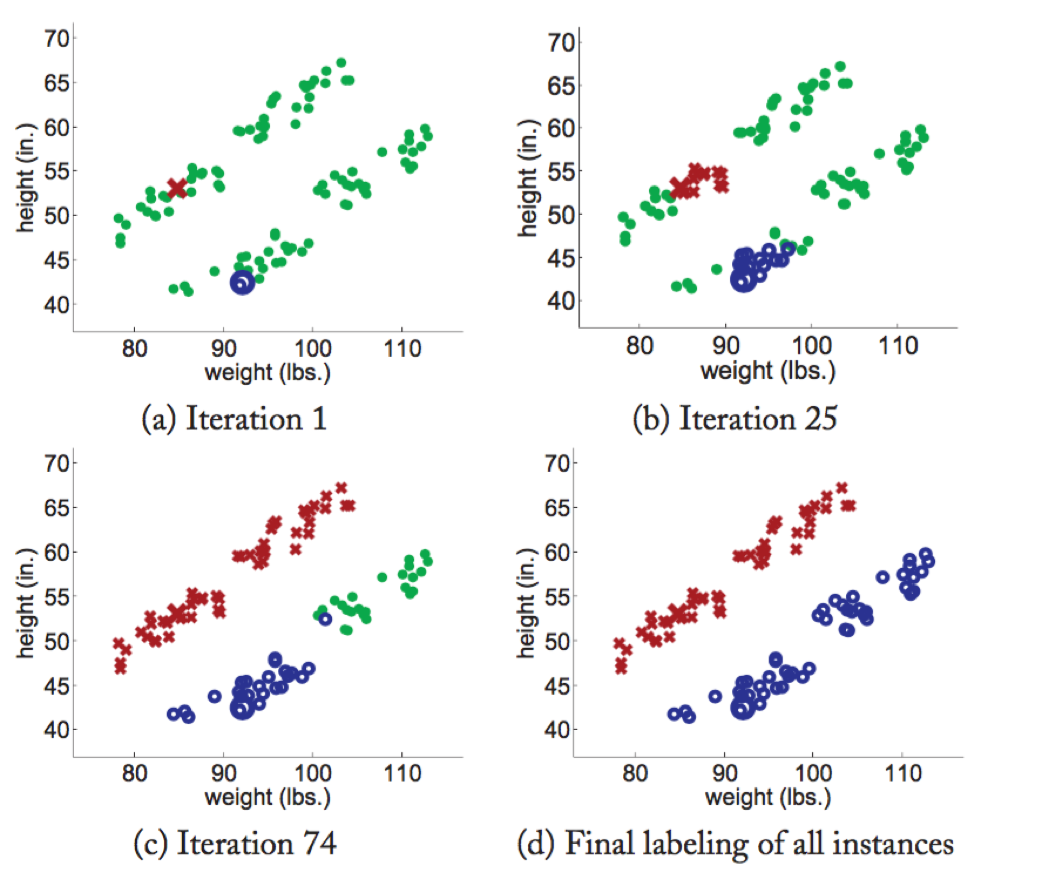
\includegraphics[width=0.9\textwidth]{res/cav.png}
      \captionsource{Korrekte Klassifiation mittels 1-nearest-neighbour}{\cite{zhu_goldberg_2009}}
  \label{fig:cav1}
\end{figure}

\begin{figure} [H]
  \centering
  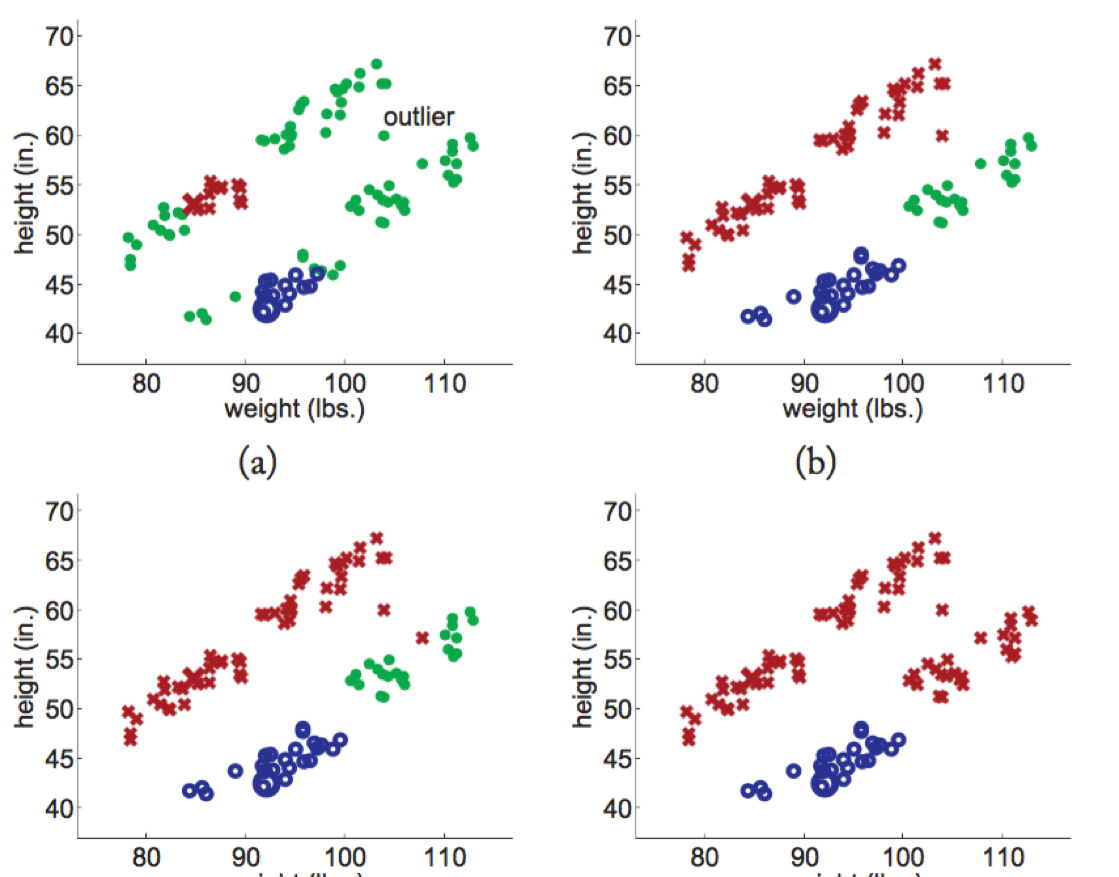
\includegraphics[width=0.9\textwidth]{res/cav2.png}
      \captionsource{Ein einziger Ausreißer führt zu falschen Ergebnissen}{\cite{zhu_goldberg_2009}}
  \label{fig:cav2}
\end{figure}


Zwar existieren gegenüber Störeinflüssen robustere Algorithmen wie \emph{k-means}, das zugrunde liegende Problem lässt sich jedoch nicht beheben. Vor jeder Anwendung dieser Verfahren müssen daher zwangsläufig die Schwächen der verwendeten Algorithmen analysiert und die möglichen Auswirkungen auf das Ergebnis bedacht werden.




%%%%%%%%%%%%%%%%%%


\clearpage{}



%\todo{Refine me}
%\commentontext{modeling}{modeling with one \enquote{l}, because of AE} 

%\section{Conclusion and Outlook}

%\subsubsection*{Acknowledgments}
%...

%In the bibliography, use \texttt{\textbackslash textsuperscript} for ``st'', ``nd'', ...:
%E.g., \enquote{The 2\textsuperscript{nd} conference on examples}.
%When you use \href{http://www.jabref.org}{JabRef}, you can use the clean up command to achieve that.



\clearpage{}


%%%%%%%%%%%%%%%%%%%%%%%%%%%%%%%%%%%%%%%%%%%%%%%%%%%%%%%%%%%%%%%%%%%%%%%%%%%%%%%
\bibliographystyle{splncs03}
\bibliography{paper}

Alle Links wurden zuletzt am 30.04.2016 überprüft.
%%%%%%%%%%%%%%%%%%%%%%%%%%%%%%%%%%%%%%%%%%%%%%%%%%%%%%%%%%%%%%%%%%%%%%%%%%%%%%%

\end{document}
